% Magda Gregorova, 2025-01-10

\chapter{Formatting}\label{ch:Format}

This chapter gives examples of some standard formatting commands and environments you may want to use.
This is far from exhaustive, there are many more things you can achieve with \LaTeX .

\section{Math Equations}\label{sec:Format_Math}

You may want to display math equations in three distinct styles: inline, numbered display, or non-numbered display.  

A formula that appears in the running text is called an inline or in-text formula. 
It is produced by the \textbf{math} environment, which can be invoked with the usual \verb|\begin{}|--\verb|\end{}| construct or with the short form \textbf{\$$\ldots$\$}.
You can use any of the symbols and structures, from $\alpha$ to $\omega$, available in \LaTeX .  

The inline style is not completely equivalent to the display style.
For example, the inline equation 
$\lim_{x\rightarrow \infty}\frac{1}{x}=0$
looks slightly different when set in the display style
\begin{equation}
    \lim_{x\rightarrow \infty}\frac{1}{x}=0 \enspace .
    \label{eq:Format_Limit}
\end{equation}

Here an example of an un-numbered equation
\begin{equation*}
    \int_{0}^{\pi/2} \cos x\,dx = \sin x\bigg\rvert_{0}^{\pi/2} = \sin
    \frac{\pi}{2} - \sin 0 = 1 \enspace .
\end{equation*}
You can use use un-numbered equations when you will not to refer to them later. 
The the first equation I can refer by its number as equation~\eqref{eq:Format_Limit}.
Note the use of \verb|\eqref| instead of \verb|\ref| here and the use of \verb|\enspace| at the end of the equation before the dot.

For a more complex equation you can use the \textbf{eqnarray} environment
\begin{eqnarray}\label{eq:Format_Longeq}
    \int_{0}^{\pi/2} \cos x\,dx & = & \sin x\bigg\rvert_{0}^{\pi/2} \nonumber \\
    & = & \sin\frac{\pi}{2} - \sin 0 = 1 \enspace .
\end{eqnarray}

\section{Tables}\label{sec:Format_Tables}

Since a table cannot be split across pages, we typically place it at the top of the page, close to its initial reference.
To achieve a proper ``floating'' placement of tables, use the environment \textbf{table} to enclose the table's contents and caption. 
The contents of the table itself have to be put inside the \textbf{tabular} environment, which ensures a suitable alignment of rows and columns.

Immediately following this sentence is the point at which Table~\ref{tab:table1} is included in the input file; compare the placement of the table here with the table in the PDF output of this document.

\begin{table}[h]
    \centering
    \caption{Frequency of Special Characters.}
    \label{tab:table1}
    \begin{tabular}{ccl}
        \toprule
        Non-English or Math&Frequency&Comments\\
        \midrule
        \O & 1 in 1,000& Swedish names\\
        $\pi$ & 1 in 5& In math\\ 
        \$ & 4 in 5 & In business\\ 
        $\Psi^2_1$ & 1 in 40,000& Unexplained\\
        \bottomrule
    \end{tabular}
\end{table}

\subsection{Figures}

Like tables, figures cannot be split across pages; the best placement for them is typically the top or the bottom of the page, close to their initial reference\footnote{The fourth, and last, footnote.}.
To ensure a proper ``floating'' placement of figures, use the environment \textbf{figure} to enclose the figure and its caption.

Figure~\ref{fig:circles} displays an image in the PDF format.
Figure~\ref{fig:star} shows a PNG image.

\begin{figure}
    \centering
    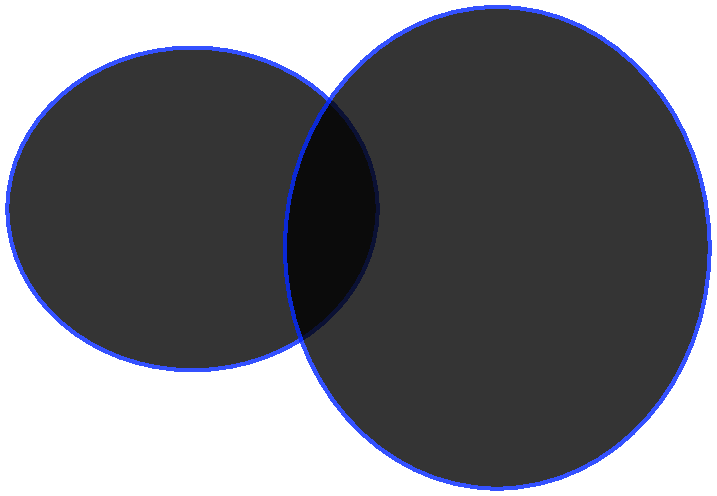
\includegraphics[scale=0.5]{circles.pdf}
    \caption{A sample circles graphic (PDF format).}
    \label{fig:circles}
\end{figure}

\begin{figure}
    \centering
    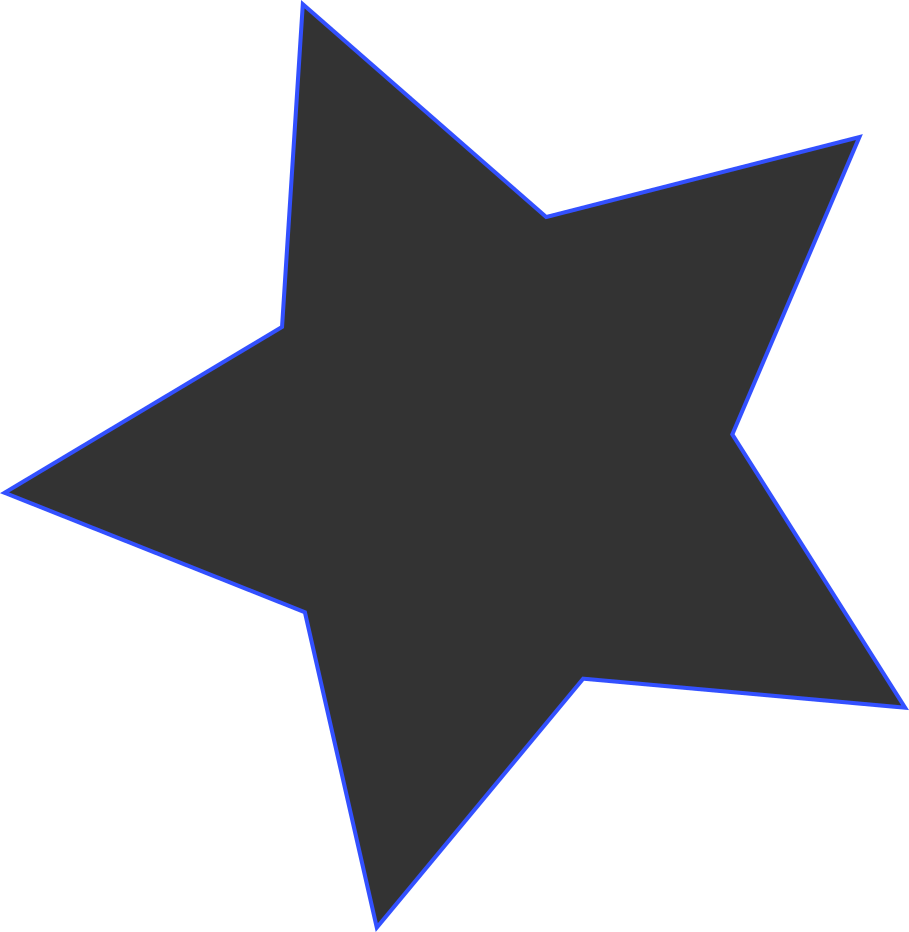
\includegraphics[scale=0.5]{star.png}
    \caption{A sample star graphic (PNG format).}
    \label{fig:star}
\end{figure}


\begin{figure}
    \centering
    \begin{subfigure}[b]{0.3\textwidth}
        \centering
        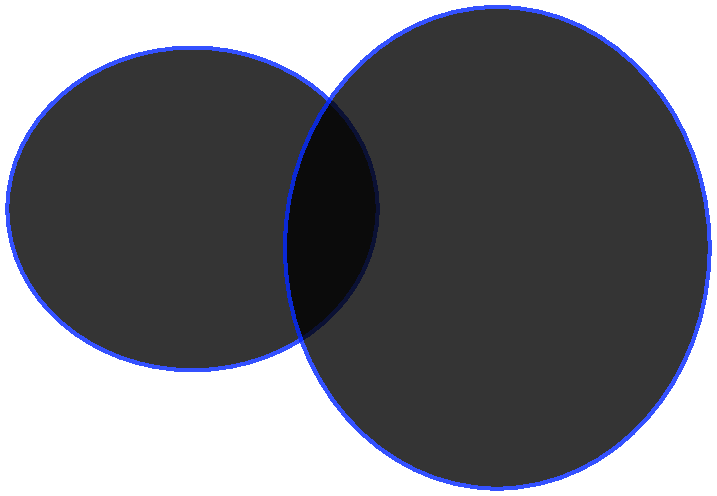
\includegraphics[width=\textwidth]{circles.pdf}
        \caption{$y=x$}
        \label{fig:circle}
    \end{subfigure}
    \hfill
    \begin{subfigure}[b]{0.3\textwidth}
        \centering
        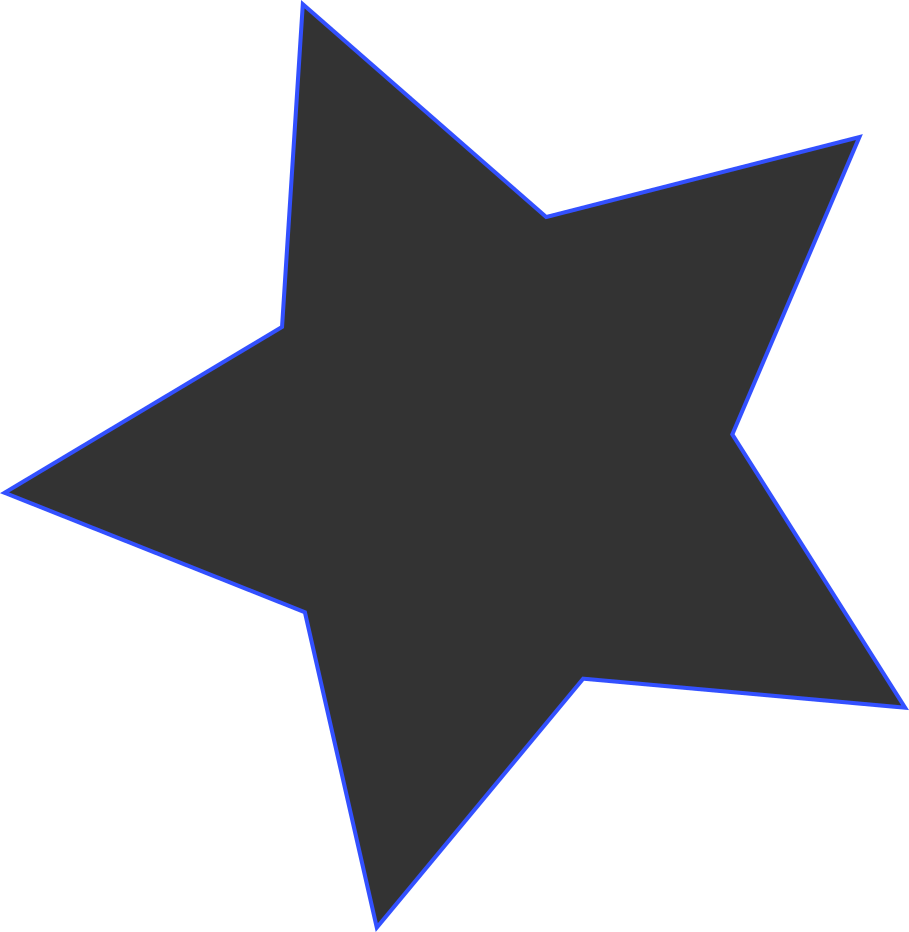
\includegraphics[width=\textwidth]{star.png}
        \caption{$y=3\sin x$}
        \label{fig:star2}
    \end{subfigure}
       \caption{Example of subfigre}
       \label{fig:two_images}
\end{figure}


\subsection{Algorithms}

To display algorithms in your document, employ the \textbf{algorithm} environment.
Algorithms can be referenced in the same way as tables and
figures (e.g., Algorithm~\ref{algo:sample}).

\begin{algorithm}
    \SetAlgoLined
    \KwData{this text}
    \KwResult{how to write an algorithm with \LaTeX}
    initialization\;
    \tcc{this is a comment to tell you that we will now really start the code}
    \While{not at end of this document}{\label{algo:sample:while}
        read the current section\;
        \eIf{understand}{
            go to the next section\;
            this section becomes the current section\;
        }{
            go back to the beginning of the current section\;
        }
    }
    \caption{How to write algorithms.}
    \label{algo:sample}
\end{algorithm}

You can reference any line of your algorithm: an example of the while loop can be seen in line~\ref{algo:sample:while}.
For more details on the \textbf{algorithm} environment, see the \url{http://tug.ctan.org/macros/latex/contrib/algorithm2e/doc/algorithm2e.pdf} document.